\question{Твердотельные лазеры. Лазер на неодимовом стекле}
Генерация осуществляется в непрерывном и импульсном режимах на переходах между 
метастабильными возбуждёнными состояниями ионов \( Nd^{3+} \). Инверсия 
достигается по четырёхуровневой системе оптической накачки.

\begin{figure}[h]
    \center
    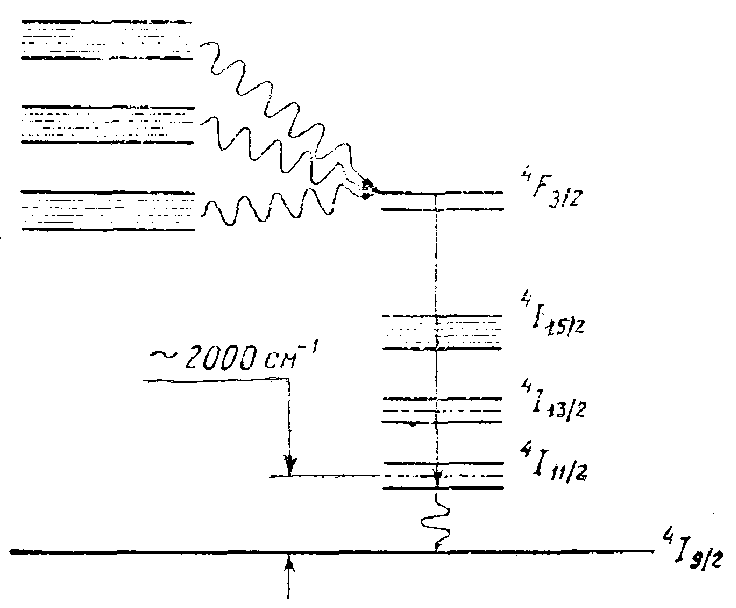
\includegraphics[width=.47\textwidth]{17}
    \caption{Уровни энергии \( Nd^{3+} \)}
\end{figure}

Стартовый уровень лазерных переходов -- метастабильный \term{4}{F}{3/2}.
Наибольшей вероятностью обладает переход \( \term{4}{F}{3/2} \rightarrow
\term{4}{I}{11/2} \). Длина волны составляет \( 1,06~\text{мкм} \).
Энергетическая щель между состояниями \term{4}{I}{11/2} и \term{4}{I}{9/2}
обеспечивает четырёхуровневый характер цикла оптической накачки.

Для достижения положительной инверсии нижний лазерный уровень должен
безызлучательно расселяться в основное состояние быстрее, чем заселяется
переходами с верхнего лазерного уровня.

Для неодимовых лазерных стёкол характерны высокая концентрация активных 
центров,сильное неоднородное уширение линии усиления, возможность получения 
активной среды в больших объёмах. Для лазеров на стекле типичен режим работы 
в одиночных импульсах высокой энергии. Однако, из-за низкой теплопроводности 
стекла такой лазер нельзя использовать в непрерывном режиме.